\documentclass{article}

\usepackage{fancyhdr}
\usepackage{extramarks}
\usepackage{amsmath}
\usepackage{amsthm}
\usepackage{amsfonts}
\usepackage{tikz}
\usepackage[plain]{algorithm}
\usepackage{algpseudocode}

\usetikzlibrary{automata,positioning}

%
% Basic Document Settings
%

\topmargin=-0.45in
\evensidemargin=0in
\oddsidemargin=0in
\textwidth=6.5in
\textheight=9.0in
\headsep=0.25in

\linespread{1.1}

\pagestyle{fancy}
\rhead{\firstxmark}
\lfoot{\lastxmark}
\cfoot{\thepage}

\renewcommand\headrulewidth{0.4pt}
\renewcommand\footrulewidth{0.4pt}

\setlength\parindent{0pt}

%
% Create Problem Sections
%

\newcommand{\enterProblemHeader}[1]{
    \nobreak\extramarks{}{Problem \arabic{#1} continued on next page\ldots}\nobreak{}
    \nobreak\extramarks{Problem \arabic{#1} (continued)}{Problem \arabic{#1} continued on next page\ldots}\nobreak{}
}

\newcommand{\exitProblemHeader}[1]{
    \nobreak\extramarks{Problem \arabic{#1} (continued)}{Problem \arabic{#1} continued on next page\ldots}\nobreak{}
    \stepcounter{#1}
    \nobreak\extramarks{Problem \arabic{#1}}{}\nobreak{}
}

\setcounter{secnumdepth}{0}
\newcounter{partCounter}
\newcounter{homeworkProblemCounter}
\setcounter{homeworkProblemCounter}{0}
\nobreak\extramarks{Problem \arabic{homeworkProblemCounter}}{}\nobreak{}

%
% Homework Problem Environment
%
% This environment takes an optional argument. When given, it will adjust the
% problem counter. This is useful for when the problems given for your
% assignment aren't sequential. See the last 3 problems of this template for an
% example.
%
\newenvironment{homeworkProblem}[1][-1]{
    \ifnum#1>0
        \setcounter{homeworkProblemCounter}{#1}
    \fi
    \section{Problem \arabic{homeworkProblemCounter}}
    \setcounter{partCounter}{1}
    \enterProblemHeader{homeworkProblemCounter}
}{
    \exitProblemHeader{homeworkProblemCounter}
}



%
% Homework Details
%   - Title
%   - Due date
%   - Class
%   - Section/Time
%   - Instructor
%   - Author
%

\newcommand{\hmwkTitle}{Homework\ \#1}
\newcommand{\hmwkName}{Fast Trajectory Replanning}
\newcommand{\hmwkDate}{February 17, 2023}
\newcommand{\hmwkClass}{CS 440: Introduction to Artificial Intelligence}
\newcommand{\hmwkClassInstructor}{Professor Abdelsam Boularias}


%
% Title Page
%

\title{
    \vspace{2in}
    \textmd{\textbf{\hmwkClass}}\\
    \textmd{\hmwkTitle\\hmwkName}\\
    \vspace{0.1in}\small{\hmwkDate}\\
    \vspace{0.1in}\large{\textit{\hmwkClassInstructor}}
    \vspace{3in}
}

\author{
    \textbf{Jay Patwardhan} {RUID}\\ 
    \textbf{Alan Wu} {208000574}\\ 
    \textbf{Neel Shejwalkar} {RUID}
}
\date{}

\renewcommand{\part}[1]{\textbf{\large Part \Alph{partCounter}}\stepcounter{partCounter}\\}

%
% Various Helper Commands
%

% Useful for algorithms
\newcommand{\alg}[1]{\textsc{\bfseries \footnotesize #1}}

% For derivatives
\newcommand{\deriv}[1]{\frac{\mathrm{d}}{\mathrm{d}x} (#1)}

% For partial derivatives
\newcommand{\pderiv}[2]{\frac{\partial}{\partial #1} (#2)}

% Integral dx
\newcommand{\dx}{\mathrm{d}x}

% Alias for the Solution section header
\newcommand{\bruh}{\textbf{\large Solution}}
\newtheorem*{solution*}{Solution}
\newenvironment{solution}{\begin{solution*}}{{\finishline} \end{solution*}}


% Probability commands: Expectation, Variance, Covariance, Bias
\newcommand{\E}{\mathrm{E}}
\newcommand{\Var}{\mathrm{Var}}
\newcommand{\Cov}{\mathrm{Cov}}
\newcommand{\Bias}{\mathrm{Bias}}

\begin{document}

\maketitle

\pagebreak

%Part 0%
\begin{homeworkProblem}
    \textbf{\large Setting Up Our Environments}\\\\

\end{homeworkProblem}

\pagebreak

%Part 1%
\begin{homeworkProblem}
    \textbf{\large Understanding the Methods}\\\\
    \part 

    Explain in your report why the first move of the agent for the example search problem is to the east rather than to the north givent hat the agent does not know initially which cells are blocked.
    \begin{figure}[h!]
			\centering
			\IfFileExists{figure1.png}{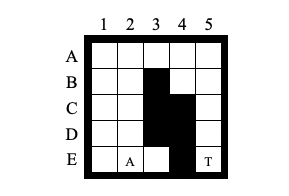
\includegraphics[width=0.5\textwidth]{figure1.png}}{No Figure Yet}
		\caption{Second Example Search Problem} 
		\end{figure}

    \begin{solution*}









    \end{solution*}

    \part

    This project argues that the agent is guaranteed to reach the target if it is not separated from it by blocked cells. Give a
convincing argument that the agent in finite gridworlds indeed either reaches the target or discovers that this is impossible
in finite time. Prove that the number of moves of the agent until it reaches the target or discovers that this is impossible is
bounded from above by the number of unblocked cells square

    \begin{solution*}
    \end{solution*}
    


   
\end{homeworkProblem}

\pagebreak

%Part 2%
\begin{homeworkProblem}
    \textbf{\large The Effects of Ties}\\\\

   
\end{homeworkProblem}

\pagebreak

%Part 3%
\begin{homeworkProblem}
    \textbf{\large Forward vs. Backward}\\\\

\end{homeworkProblem}

\pagebreak

%Part 4
\begin{homeworkProblem}
    \textbf{\large Heuristics in the Adaptive $A ^{*}$}\\\\

    
\end{homeworkProblem}

\pagebreak

%Part 5
\begin{homeworkProblem}
    \textbf{\large Heuristics in the Adaptive $A ^{*}$}\\\\

    
\end{homeworkProblem}
\pagebreak
%Part 6%
\begin{homeworkProblem}
    \textbf{\large Statistical Significance}\\\\


\end{homeworkProblem}

\end{document}